\chapter{Spinrendszerek statisztikus fizikai alapjai, negat\'{\i}v h\H{o}m\'ers\'eklet, Pa\-ra\-m\'ag\-ne\-ses--fer\-ro\-m\'ag\-ne\-ses \'at\-me\-net, kritikus viselked\'es}
 
 \section{Spinrendszerek leírásának alapja}
  
  Klasszikusan statisztikus fizikai módon nem értelmezgető a mágnesezettség, mint a töltött részecskék pályamomentuma. A Hamilton-függvény: $H=\suml{i=1}{f}\frac{1}{2m}\big(\pv_i+q\Av_i\big)^2+\frac{1}{2}\suml{i\ne j}{f}V(\rv_i-\rv_j)$, mellyel az állapotszám: $Z=\frac{1}{h^{dN}N!}\intl{}{}\dd^{dN}r\dd^{dN}p\,e^{-\beta H}$. Itt a $\pv_i$ szerinti integrálok Gauss-integrálok, melyeket el lehet végezni, így az állapotösszeg független lesz $\Av$-től, vagyis $m=\frac{1}{\beta}\pder{\ln Z}{B}=0$.
  
  Mi lokalizált momentumok mágneses viselkedését fogjuk leírni, ahol a \eqref{eq:03-SCHem} egyenletből csak a Pauli-tagot vesszük figyelembe, és a Hund-szabályok miatt
  \al{
    \opH=\suml{i}{}\opH_i=\suml{i}{}\mu_\text{B}\frac{1}{\hbar}gB\opS^z_i,
   }
   ahol $g$ a Landé-faktor, $\mu_\text{B}$ a Bohr-magneton, és $B$ a mágneses tér erőssége. $\opS^z_i$ itt az $i$-edik lokalizált momentum spinoperátorának $z$-edik komponense.
  
  A kölcsönhatások leírásához nem ismertetjük a lezajló mechanizmusokat, hanem egy modellt fogunk vizsgálni. A kölcsönható Ising-modell Hamilton-függvénye:
  \al{
   H=-J\suml{\mv{i,j}}{}s_is_j-h\suml{i}{}s_i,
  }
  ahol $J$ a kölcsönhatás erőssége (kicserélődési csatolás). Ha $J>0$ akkor ferromágneses, ha $J<0$ akkor antiferromágneses a csatolás, $h$ pedig a külső mágneses térnek megfelelő tag. A kölcsönhatás minden első szomszéd rácshely között történik, a rács pedig $d$ dimenziós négyzetrács. A rácshelyeken Ising-spinek vannak, melyeknek értéke $\pm1$ lehet. 
  
  Ahhoz, hogy összhangban legyünk a előző felírással látjuk, hogy $h=-\frac{1}{2}\mu_\text{B}gB$-t kell választani.
  
  \subsection{Nemkölcsönható spinrendszerek}
   
   Nemkölcsönható esetben $J=0$, vagyis
   \al{
    \opH_i=-h \suml{i}{}s_i.
   }
   A kanonikus állapotösszeg:
   \al{
    Z_1
     &=\tr e^{-\beta H_i}
      =\tr e^{\beta s_i h}
      =\suml{s=-1,1}{} e^{\beta h s}
      =e^{-\beta h}+e^{\beta h}
      =2\ch\left(\beta h\right)\\
     Z&=Z_1^N\\
     F&=-k_\text{B}T\ln Z
       =-k_\text{B}TN\ln Z_1
       =-k_\text{B}TN\ln \left[2\ch\left(\beta h\right)\right]\\
     M&=\frac{1}{\beta}\pder{\ln Z}{h}
       =\frac{N}{\beta}\pder{\ln Z_1}{h}
       =\frac{N}{\beta} \frac{1}{2\ch\left(\beta h\right)}\cdot 2\sh\left(\beta h\right)\cdot \beta
       = N\tgh\left(\beta h\right)\\
     \chi
      &=\pder{M}{h}
       =N\beta\frac{1}{\ch^2\left(\beta h\right)}.
   }
   A szuszceptibilitás képletében $B\to 0$-ra $\chi\sim\frac{1}{T}$, ami a Curie--Weiss-törvény. Minden véges $T$-re $\chi>0$, így a paramágneses állapot stabil. 
   
   \begin{figure}[ht!]
    \centering
     \subfloat[\label{fig:B08-1}]{\begin{overpic}[width= 0.45\textwidth]{./B08tetel/chi-t}
        \put(55,20){\tikz \draw[-latex,line width=1.3pt,red] (1,1) node[above right] {$h$ növekszik} .. controls (0.75,0.85) and (0.2,0.6) .. (0,0);}
       \end{overpic}}
     \hspace{6pt}
     \subfloat[\label{fig:B08-11}]{\begin{overpic}[width= 0.45\textwidth]{./B08tetel/m-h}
        \put(130,70){\tikz \draw[-latex,line width=1.3pt,red] (0,1.6) .. controls (0.2,0.5) and (1,0.1) .. (1.3,0) node[below] {$T$ növekszik};}
       \end{overpic}}
    \caption{A szuszceptibilitás a hőmérséklet függvényében különböző mágneses tér mellett (a), illetve a mágnesezettség a külső tér függvényében különböző hőmérsékleten (b).}
   \end{figure}
   
  \subsection{Negatív hőmérséklet}\label{ss:neghom}
   
   Tekintsünk egy véges állapotú rendszert. Ennek az állapotszáma az összenergiának nem monoton növő függvénye, mert hatalmas energiákon a rendszer úgyis nagyon nagy valószínűséggel a legmagasabb energiájú állapotban lesz, vagyis az állapotszáma újra kicsi lesz, az csökkenni fog egy korábbi értékhez képest. Normál rendszere $\ln\Omega\approx\ln\omega(E)\sim S$, így ha $\pder{\Omega}{E}<0$ $\Rightarrow$ $\pder{S}{E}=\frac{1}{T}<0$, ami nem értelmezhető.
   
   Egy konkrét példa legyen az előző kétállapotú nemkölcsönható rendszer. Álljon $N$ spinből a rendszer, amiből $N_+$ van az $E_+=h$ és $N_-$ van az $E_-=-h$ állapotban. $N_+$ és $N_-$ kifejezve a mágnesezettséggel és a részecskeszámmal: $N_\pm=\frac{N\pm M}{2}$. Ezzel a teljes energia: $E=h(N_+-N_-)=hM$. Az állapotszám:
   \al{
    \Omega=\frac{N!}{N_+!N_-!}=\frac{N!}{\left(\frac{N+M}{2}\right)!\left(\frac{N-M}{2}\right)!}.
   }
   Innen az entrópia, mintha normál rendszerrel lenne dolgunk, felhasználva a Stirling-formulát ($\ln x!\approx x\ln x-x$):
   \al{
    S&=k_\text{B}\ln\Omega
      \approx k_\text{B}
       \left(
        N\ln N-N
        -\frac{N+M}{2}\ln\frac{N+M}{2}+\frac{N+M}{2}
        -\frac{N-M}{2}\ln\frac{N-M}{2}+\frac{N-M}{2}
       \right)\\
     &= k_\text{B}
       \left(
        N\ln N
        -\frac{N+M}{2}\ln\frac{N+M}{2}
        -\frac{N-M}{2}\ln\frac{N-M}{2}
       \right)\\
     &= k_\text{B}
       \left(
        \frac{N+M}{2}\ln N+\frac{N-M}{2}\ln N
        -\frac{N+M}{2}\ln\frac{N+M}{2}
        -\frac{N-M}{2}\ln\frac{N-M}{2}
       \right)\\
     &= -k_\text{B}
       \left(
        \frac{N+M}{2}\ln\frac{N+M}{2N}
        +\frac{N-M}{2}\ln\frac{N-M}{2N}
       \right)
   }
   \al{
    \frac{1}{T}
     &=\pder{S}{E}
      =\frac{1}{h}\pder{S}{M}\\
     &=-\frac{k_\text{B}}{h}
       \left(
        \frac{1}{2}\ln\frac{N+M}{2N}
        +\frac{N+M}{2}\frac{2N}{N+M}\frac{1}{2N}
        -\frac{1}{2}\ln\frac{N-M}{2N}
        +\frac{N+M}{2}\frac{2N}{N-M}\frac{-1}{2N}
       \right)\\
     &=-\frac{k_\text{B}}{2h}\ln\frac{N+M}{N-M}
      =\frac{k_\text{B}}{2h}\ln\frac{N_-}{N_+}.
   }
   Itt $T>0$, ha $N_->N_+$, de ha fordítva van, akkor $T<0$ (\ref{fig:B08-NegT}. ábra). Ha $N_+>N_-$, akkor megvalósul az inverz populáció. Természetesen ez nem egy termodinamikai egyensúlyi állapot. Ilyen akkor áll fenn, ha a rendszer erősen kölcsönhat a környezettel, pl. lézerek pumpálása. 
   \begin{figure}[ht!]
    \centering
    \subfloat[\label{fig:B08SE}]{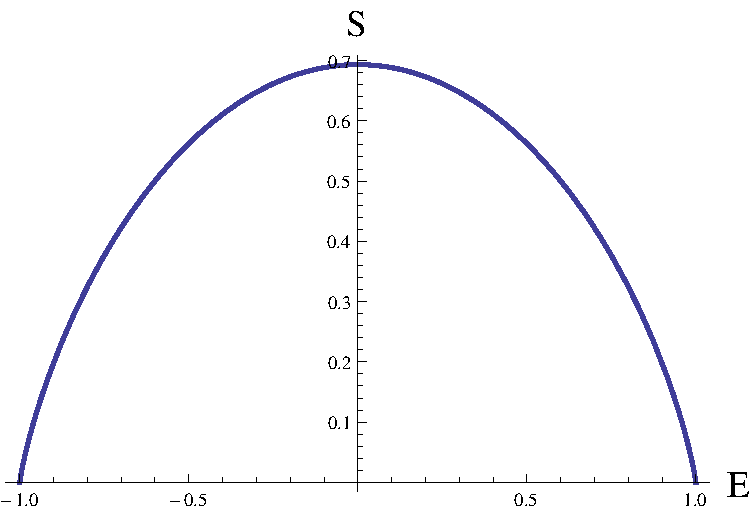
\includegraphics[width=0.45\textwidth]{./B08tetel/S-E}} \hspace{6pt}
    \subfloat[\label{fig:B08-T-E}]{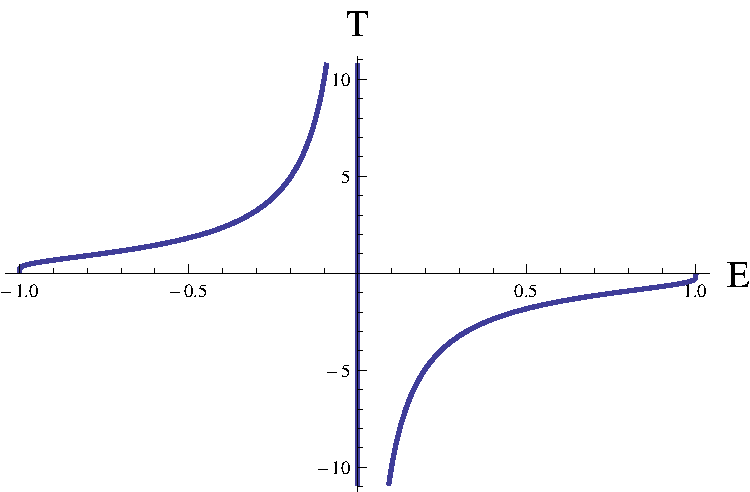
\includegraphics[width= 0.45\textwidth]{./B08tetel/T-E}} 
    \caption{A véges állapotú spinrendszer esetében számolt entrópia és hőmérséklet.}\label{fig:B08-NegT}
   \end{figure}
   
   
    
  \subsection{Kölcsönható spinrendszerek}
   
   Most legyen $J>0$, azaz tekintsünk ferromágneses csatolást. A Hamilton-függvényt átírhatjuk:
   \al{
    H=-\frac{J}{2}\suml{i,j}{}s_is_j-h\suml{i}{}s_i
     =-\suml{i}{}\left(h+\frac{J}{2}\suml{j}{}s_j\right)s_i.
     =-\suml{i}{}h_{\text{eff},i}s_i.
   }
   Itt $h_{\text{eff},i}$-re átlagolni fogunk. A rendszer vizsgálatakor átlagokat képezünk az összes spinkonfigurációra. Mivel ezt nem tudjuk elvégezni, ezért egy spint rögzítünk, és az összes ilyen konfigurációra átlagolunk ki, és azt a kitüntetett spint az átlagolt többi spin közé tesszük vissza, és nézzük a kölcsönhatást. Ez itt:
   \al{
    \mv{h_{\text{eff},i}}
     =\mv{h+\frac{J}{2}\suml{j}{}s_j}
     =h+\frac{Jz}{2}\frac{M}{N},
   }
   ahol $\frac{M}{N}$ az mágnesezettségi sűrűség $m$, $z$ pedig a koordinációs szám. Ha ezt az átlagtér Hamilton-függvényt használjuk, akkor egy effektíve nemkölcsönható rendszer kapunk csak más $h$-val. A fentieknek megfelelően az állapotegyenlet:
   \aln{
    m=\tgh\left(\beta\left(h+\frac{Jz}{2}m\right)\right).\label{eq:B08-alle}
   }
   Ez megoldható $h$-ra: $h=\frac{1}{\beta}\arcth(m)-\frac{Jz}{2}m$, ahonnan a szuszceptibilitás inverze:
   \al{
    \chi^{-1}=\pder{h}{m}=\frac{k_\text{B}T}{1-m^2}-\frac{Jz}{2}.
   }
   A fázis stabilitásának feltétele: $0<\chi^{-1}$. 
   
   Ha $h=0$, a paramágneses fázisban $m=0$. Ez instabil lesz, ha csökkentjük a hőmérsékletet: $k_\text{B}T_C=\frac{Jz}{2}$ hőmérsékleten. Ekkor a ferromágneses állapot fog stabillá válni: $m\ne 0$ véges mágnesezettséggel. Nézzük meg, hogy ez tényleg stabil-e. Ehhez szükséges, hogy 
   \al{
    0&<\frac{k_\text{B}T}{1-m^2}-\frac{Jz}{2}\\
    \beta\frac{Jz}{2}&<\frac{1}{1-m^2}\\
    \beta\frac{Jz}{2}m&<\frac{m}{1-m^2}\\
    \beta\frac{Jz}{2}m&<\frac{m}{1-\tgh^2\left(\beta\frac{Jz}{2}m\right)}
     =\ch\left(\beta\frac{Jz}{2}m\right)\sh\left(\beta\frac{Jz}{2}m\right)\\
    x&<\ch(x)\sh(x),
   }
   ami pedig mindig igaz. Így valóban stabillá válik a ferromágneses állapot a paramágnesessel szemben, így történik egy átalakulás. 
   
   Az állapotegyenlet megoldása grafikus módszerrel szemléletesen megadható, ezt \aref{fig:B08-grafikusmego}. ábra mutatja.
   \begin{figure}[ht!]
    \centering
    \subfloat[\label{fig:B08mt}]{\begin{overpic}[width=0.45\textwidth]{./B08tetel/m-T-grafikusmegoldas}
        \put(120,100){\tikz \draw[-latex,line width=1.3pt,red] (0,3) .. controls (0.15,1.5) and (0.4,0.4) .. (1.6,0)node[below] {$T$ növekszik};}
       \end{overpic}} \hspace{6pt}
    \subfloat[\label{fig:B08mh}]{\begin{overpic}[width=0.45\textwidth]{./B08tetel/m-h-grafikusmegoldas}
        \put(120,100){\tikz \draw[-latex,line width=1.3pt,red] (0.3,0) node[below right] {$h$ növekszik} .. controls (0,0.3) and (-0.4,1.5) .. (-0.5,2.5);}
       \end{overpic}} 
    \caption{Az állapotegyenlet jobb és bal oldalát ábrázoltuk $m$ függvényében. Ahol a két oldal egyenlő, ott lesz megoldás.}\label{fig:B08-grafikusmego}
   \end{figure}
   
   
  \subsection{Kritikus viselkedés}
   
   Vizsgáljuk meg a termodinamikai mennyiségeket $T_C$ közelében. az Ising-modell esetében. 
   
   $h=0$-ra $T_\text{C}$ közelében $m\to 0$. \Eqaref{eq:B08-alle} egyenlet alapján $m$ hőmérsékletfüggése:
   \al{
    m&=\tgh\left(\frac{T_\text{C}}{T}m\right)
      \approx \frac{T_\text{C}}{T}m-\frac{1}{3}\left(\frac{T_\text{C}}{T}m\right)^3\\
    1&=\frac{T_\text{C}}{T}+\frac{1}{3}\frac{T^3_\text{C}}{T^3}m^2\\
    m^2&=\frac{1-\frac{T_\text{C}}{T}}{\frac{1}{3}\frac{T^3_\text{C}}{T^3}}
       =3\frac{T^2}{T^2_\text{C}} \abs{1-\frac{T}{T_\text{C}}}\\
    m&\sim\abs{1-\tau}^{\frac{1}{2}},
   }
   vagyis $\beta=\frac{1}{2}$.
   
   A $\chi$ hőmérsékletfüggése:
   \al{
    \chi^{-1}
     &=\frac{k_\text{B}T}{1-m^2}-\frac{Jz}{2}
      =\frac{k_\text{B}T}{1-m^2}-k_\text{B}T_\text{C}
      \approx k_\text{B}(T-T_\text{C})\\
     \chi&\sim \abs{T-T_\text{C}}^{-1},
   }
   vagyis $\gamma=1$. 
   
   A $m$ $h$-tól való függése $T=T_\text{C}$-n:
   \al{
    h&=k_\text{B}T_\text{C}\arcth(m)-k_\text{B}T_\text{C}m
     \approx k_\text{B}T_\text{C}\left(m+\frac{1}{3}m^3\right)-k_\text{B}T_\text{C}m
     =\frac{k_\text{B}T_\text{C}}{3}m^3\\
    m&\sim \abs{h}^{\frac{1}{3}},
   } 
   vagyis $\delta = 3$.
   
   
%    {\color{red} A fajhős exponens még jó lenne, nem tudom hogyan lehetne a lehető legkevesebb munkával kihozni\dots}
%    A fajhő számolásához szükségünk van a szabadenergia sűrűségre:
%    \al{
%     &m=-\pder{f}{h}
%     &\Rightarrow
%     &&f=
%    }
   
   
   
   
   
   
   
   
   
   
   
   
   
   
   